\documentclass{article}
\usepackage{graphicx} % Required for inserting images
\usepackage{amsmath}
\usepackage{amssymb}
\usepackage{amsthm}
\usepackage{amsfonts}
\usepackage[english]{babel}
\usepackage{caption}
\usepackage{subfigure}
\usepackage{subcaption}

\newtheorem{theorem}{Theorem}
\newtheorem{question}{Question}
\newtheorem{lemma}{Lemma}

\title{The Minimum LCM of a sequence}
\author{Daniel Mineev}

\begin{document}

\maketitle

\section{Introduction}

Here, I would like to discuss the problem of minimizing the LCM of a sequence of \(k\) \textbf{distinct} integers given their exact sum to be \(n\). This value I will denote as \(L_K(N)\). I will establish a lower and an upper bound on this value for any \(n, k \in \mathbb{N}\). The lower bound, as you will see, is extremely simple to establish; a far more complex problem is establishing an upper bound.
\begin{theorem}
	\(L_k(n) \geq n / \left( \frac{1}{1} + \frac{1}{2} + \ldots + \frac{1}{k} \right) \)
\end{theorem}
Consider the following problem, listed in the shortlist for IMO 2022, as an example of where this function has been used.
\begin{question}
	A number is called Norwegian if it has three distinct positive divisors whose sum is equal to 2022. Determine the smallest Norwegian number. \\
	(Note: The total number of positive divisors of a Norwegian number is allowed to be larger than 3.)
\end{question}
This problem is equivalent to calculating the exact value of \(L_3(2022)\), it is specifically this problem, which convinced me to generalize the concept.

\section{Lower Bound}

Here, I will prove that the lower bound on the value of \(L_k(n)\) is \(n /  \left( \frac{1}{1} + \frac{1}{2} + \ldots + \frac{1}{k} \right) \), along with the fact that this bound is tight.

\begin{theorem}
	\(L_k(n) \geq n / \left( \frac{1}{1} + \frac{1}{2} + \ldots + \frac{1}{k} \right) \)
\end{theorem}

\renewcommand\qedsymbol{$\blacksquare$}

\begin{proof}
Let us assume the opposite, that indeed, \(L_k(n) < n /  \left( \frac{1}{1} + \frac{1}{2} + \ldots + \frac{1}{k} \right) \), then let \(L_k(n)/a_1 < L_k(n)/a_2 < \ldots <  L_k(n) / a_k\) be the \(k\) divisors of \(L_k(n)\) (meaning, the \(k\) divisors, which sum to \(n\), from the definition), then we conclude, that,
\begin{multline}
	n = \sum_{i = 1}^k \frac{L_k(n)}{a_i} = L_k(n) \left( \frac{1}{a_1} + \frac{1}{a_2} + \ldots + \frac{1}{a_k} \right) 
	\\ < \frac{n}{\frac{1}{1} + \frac{1}{2} + \ldots + \frac{1}{k}} \left( \frac{1}{a_1} + \frac{1}{a_2} +  \ldots + \frac{1}{a_k} \right)
\end{multline}
However, as one can probably already see, \(\frac{1}{a_1} + \frac{1}{a_2} +  \ldots + \frac{1}{a_k} \leq \frac{1}{1} + \frac{1}{2} + \frac{1}{3} + \ldots + \frac{1}{k}\), however even if this sum equals its maximum possible value the last expression will only be \(n\), thus it is impossible for there to be a strict less sign in the inequality, contradiction. Thus, the inequality is indeed true.
\end{proof}

Notice that the lower bound on \(L_k(n)\) gives something more interesting. Obviously one can see that from this, one can conclude that,
\begin{equation}
	[a_1, a_2, \ldots, a_k] \geq \frac{1}{\frac{1}{1} + \frac{1}{2} + \ldots + \frac{1}{k}} \sum_{i = 1}^k a_i
\end{equation}
is true for any \(a_1, \ldots, a_k \in \mathbb{N}\), assuming that for no two \(a_i, a_j\) we have \(a_i = a_j\). As a small example of the two equations, we get the following nice simple tricks, (given, that \(a \neq b\))
\begin{gather}
	[a, b] \geq \frac{2}{3}(a + b) \\
	(a, b) = \frac{ab}{[a, b]} \leq \frac{2ab}{3(a + b)}
\end{gather}
This is a direct consequence, of the lower bound of \(L_2(N)\), which is \(L_2(N) \leq \frac{2}{3} N\).

\section{Upper Bound}

\subsection{\(L_2(N)\) Analysis}

Let us try to calculate the precise value of \(L_2(N)\).

\begin{theorem}
	Given \(n \in \mathbb{N}\), that \(n \geq 3\), the value of \(L_2(N)\) is \((q - 1)r\), where \(q\) is the smallest divisor of \(N\) greater than \(2\) (this is achieved by the partitioning, \(\frac{n}{q}, n - \frac{n}{q}\)).
\end{theorem}

\begin{proof}
	Let us assume this is not the case, then it must hold, that, the partition of \(n\) was into two parts \(xd\) and \(yd\), where \(x, y > 1\), and \(d\) is the greatest common denominator of the two numbers in the partition (consequently \((x, y) = 1\)). Notice, that \([xd, yd] = d[x, y]\), however, due to \((x, y) = 1\), one can conclude that \([x, y] = xy\), thus \([xd, yd] = xyd\). However, notice, that \(xy\) is minimized, when \(x = 2\) and \(y = \frac{n}{d} - 2\), but notice that even then,

\begin{equation}
	dxy = 2d \biggl( \frac{n}{d} - 2 \biggr) = 2(n - d)
\end{equation}

However, notice, that, if one considers the partition where \(x = 1\) and \(y = \frac{n}{d} - 1\), then the least common multiple will be the following,
\begin{equation}
	dxy = d \biggl( \frac{n}{d} - 1 \biggr) = n - d
\end{equation}
Which is better, than than \(2(n - d)\), consequently, it is always benificial to make the partition of the form \(d, dx\), thus, to minimize the least common denominator, the value of \(dx\), must be minimized, in other words the value of \(\frac{n}{d} - 1\) must be minimized, however this problem is equivelent to maximizing \(d\) (note, that the maximized value of \(d\) is represented as \(r\) in the statement). However, to simplify the statement, notice that maximizing \(d\) means minimizing \(\frac{n}{d}\), however \(\frac{n}{d} \geq 3\) must hold, for the partitioning to be legal (e.i. the numbers would be distinct), consequently, one sees, that if \(q\) is the smallest divisor, such that \(q \geq 3\), the value of \(L_2(N)\) is exactly \((q - 1)r\).
\end{proof}

Notice, that trivially (through simply considering the partitioning \(1, n - 1\)), \(L_2(N)\) is at least bounded by \(N - 1\), however through this theorem, we understand that this bound is tight for prime values of \(N\), thus proving, that indeed, the upper bound \(N - 1\) is tight.

While this does indeed already tell us a lot, the function is bounded by two linear functions, consequently \(L_2(N) = O(N)\), however this does not tell the full story, the question that I will raise in this section, will be to find a function \(\widehat{L}_2(N)\), such that,
\begin{equation}
	\biggl[ \sum_{k = 1}^N L_2(k) \biggr] / N = \biggl[ \sum_{k = 1}^N \widehat{L}_2(k) \biggr] / N
\end{equation}
In simple terms, a nice approximation of \(L_2(N)\) in the form of a linear function, \(\widehat{L}_2(N)\). To start the analysis, I will perform a common trick, notice, that \(L_2(N)\) from the previous theorem is a very hard function to work with, consequently to eliminate any drastic changes in the value of the function, I propose analysing the value of the following,
\begin{equation}
	AL_2(N) = \biggl[ \sum_{k = 1}^N L_2(k) \biggr] / N
\end{equation}

Notice, that the problem of identifing the smallest divisor greater than 2, is not extremely different from identifying the smallest prime divisor, this is due to the fact, that the smallest divisor greater than 2, must be part of the set \(\{4, 3, 5, 7, \ldots\}\) (in other words, the union of \(\{4\}\) and the set of primes, greater than 2)
let $\pi_n$ represent the probability that the $n$-th special number is the minimal divisor greater than 2, then, indeed, a recursive relationship holds (where $s_n$ is the $n$-th special number),

\begin{equation}
	\pi_n = \frac{1}{s_n}\left( 1 - \sum_{i = 1}^{n - 1}\pi_i \right) = \frac{\pi_{n - 1}(s_{n - 1} - 1)}{s_n}
\end{equation}

The last transition comes from,

\begin{multline}
	 1 - \sum_{i = 1}^{n - 2} \pi_i  = \pi_{n - 1} s_{n - 1} 
	 \\ \implies 1 - \sum_{i = 1}^{n - 1}\pi_i = \pi_{n - 1}s_{n - 1} - \pi_{n - 1} = \pi_{n - 1}(s_{n - 1} - 1)
\end{multline}

Now, all that is left, to reiterate the recursive relationship to obtain,

\begin{equation}\label{problamatic_moment_1}
	\pi_n = \frac{(s_1 - 1) \cdot (s_2 - 1) \ldots (s_{n - 1} - 1)}{s_1 \ldots s_n} = \frac{1}{s_1} \prod_{i = 1}^{n - 1} \frac{s_i - 1}{s_i} 
\end{equation}

First of all, quick note, from this, one can conclude, that, $\pi_n \leq \frac{1}{s_n}$, which has as a direct biproduct,
\begin{equation}
	\lim_{n \rightarrow \infty} \pi_n = 0
\end{equation}

Now, I shall return to the definition of \(AL_2(N)\), to get, (where, \(d(k)\) represents the smallest divisor, which is greater than 2 of \(k\))

\begin{multline}
	AL_2(N) = \biggl[ \sum_{k = 1}^N L_2(k) \biggr] / N =  \biggl[ \sum_{k = 1}^N k - \frac{k}{d(k)} \biggr] / N 
	\\ = \biggl[ \frac{N(N + 1)}{2} \biggr] / N - \sum_{k = 1}^N \frac{k}{N d(k)} = \frac{N + 1}{2} - \mathbb{E} \biggl[ \frac{k}{d(k)} \biggr]
\end{multline}

The expectation is just a convienient way to rephrase the previous, assuming that the random variable \(k\) is uniformly selected from \(1\) to \(N\). Thus, I propose analysing that value,

\begin{equation}
	\mathbb{E} \biggl[ \frac{k}{d(k)} \biggr] = \sum_{k = 1}^{\infty} \frac{\pi_k N}{2 s_k} \leq N \sum_{k = 1}^{\infty} \frac{1}{s_k} \cdot \frac{1}{2 s_k} = N \sum_{k = 1}^{\infty} \frac{1}{2 s_k^2}
\end{equation}

One of the methods here, is to immediately write the last expression using the prime zeta function,

\begin{equation}
	\sum_{k = 1}^{\infty} \frac{1}{2 s_k^2} = \frac{1}{32} + \left[ P(2) - \frac{1}{4} \right] / 2 \approx \frac{1}{32} + \left[ 0.45224 - \frac{1}{4} \right] / 2 \approx 0.13237
\end{equation}

Thus, in the end, we have, that,

\begin{multline}
	AL_2(N) = \frac{N + 1}{2} - \mathbb{E} \biggl[ \frac{k}{d(k)} \biggr] \approx \frac{N + 1}{2} - 0.13237 N \approx 0.36763 N
\end{multline}

However, I have found this result to not be precise enough, this is due to the rough approximation we make, for the value of \(\pi_k\), it far from accurate, I am referencing this specific moment in logic,

\begin{equation}
	\frac{1}{s_n} \prod_{i = 1}^{n - 1} \frac{s_i - 1}{s_i} \leq \frac{1}{s_n}
\end{equation}

If one accounts for this error (I have not figured out a way here, to get a nice formula to simplify the last, thus I have simply calculated this with a computer),

\begin{equation}
	\sum_{k = 1}^{\infty} \frac{\pi_k}{s_k}  = \sum_{k = 1}^{\infty} \biggl[ \frac{1}{s_n} \prod_{i = 1}^{n - 1} \frac{s_i - 1}{s_i} \cdot \frac{1}{s_k} \biggr] \approx 0.18959 = C
\end{equation}
From, one concludes, that,

\begin{multline}
	AL_2(N) = \frac{N + 1}{2} - \mathbb{E} \biggl[ \frac{k}{d(k)} \biggr] = \frac{N + 1}{2} - N \sum_{k = 1}^{\infty} \frac{1}{2 s_k^2}
    \\ \approx \frac{N + 1}{2} - \frac{N}{2} \cdot C \approx \left( \frac{1 - C}{2} \right) N \approx 0.405205 N
\end{multline}

Thus, we have come to quite an accurate formula for \(AL_2(N)\), which is \(AL_2(N) \approx 0.405 N\), let the constant be \(c\), then, one can conclude, the following,

\begin{gather}
    cN = \biggl[ \sum_{k = 1}^N L_2(k) \biggr] / N \implies c N^2 = \sum_{k = 1}^N L_2(k) \\
    c(N - 1) = \biggl[ \sum_{k = 1}^{N - 1} L_2(k) \biggr] / (N - 1) \implies c (N - 1)^2 = \sum_{k = 1}^{N - 1} L_2(k) \\
    \implies \sum_{k = 1}^N L_2(k) - \sum_{k = 1}^{N - 1} L_2(k) = L_2(N) = cN^2 - c(N - 1)^2 = 2cN - c
\end{gather}
Thus, we get, that \(L_2(N) \approx 0.81041 N - 0.405205\), in other words, with large values of \(N\), the approximate value is around \(0.81041 N\)

\begin{figure}[htbp]
    \centering
    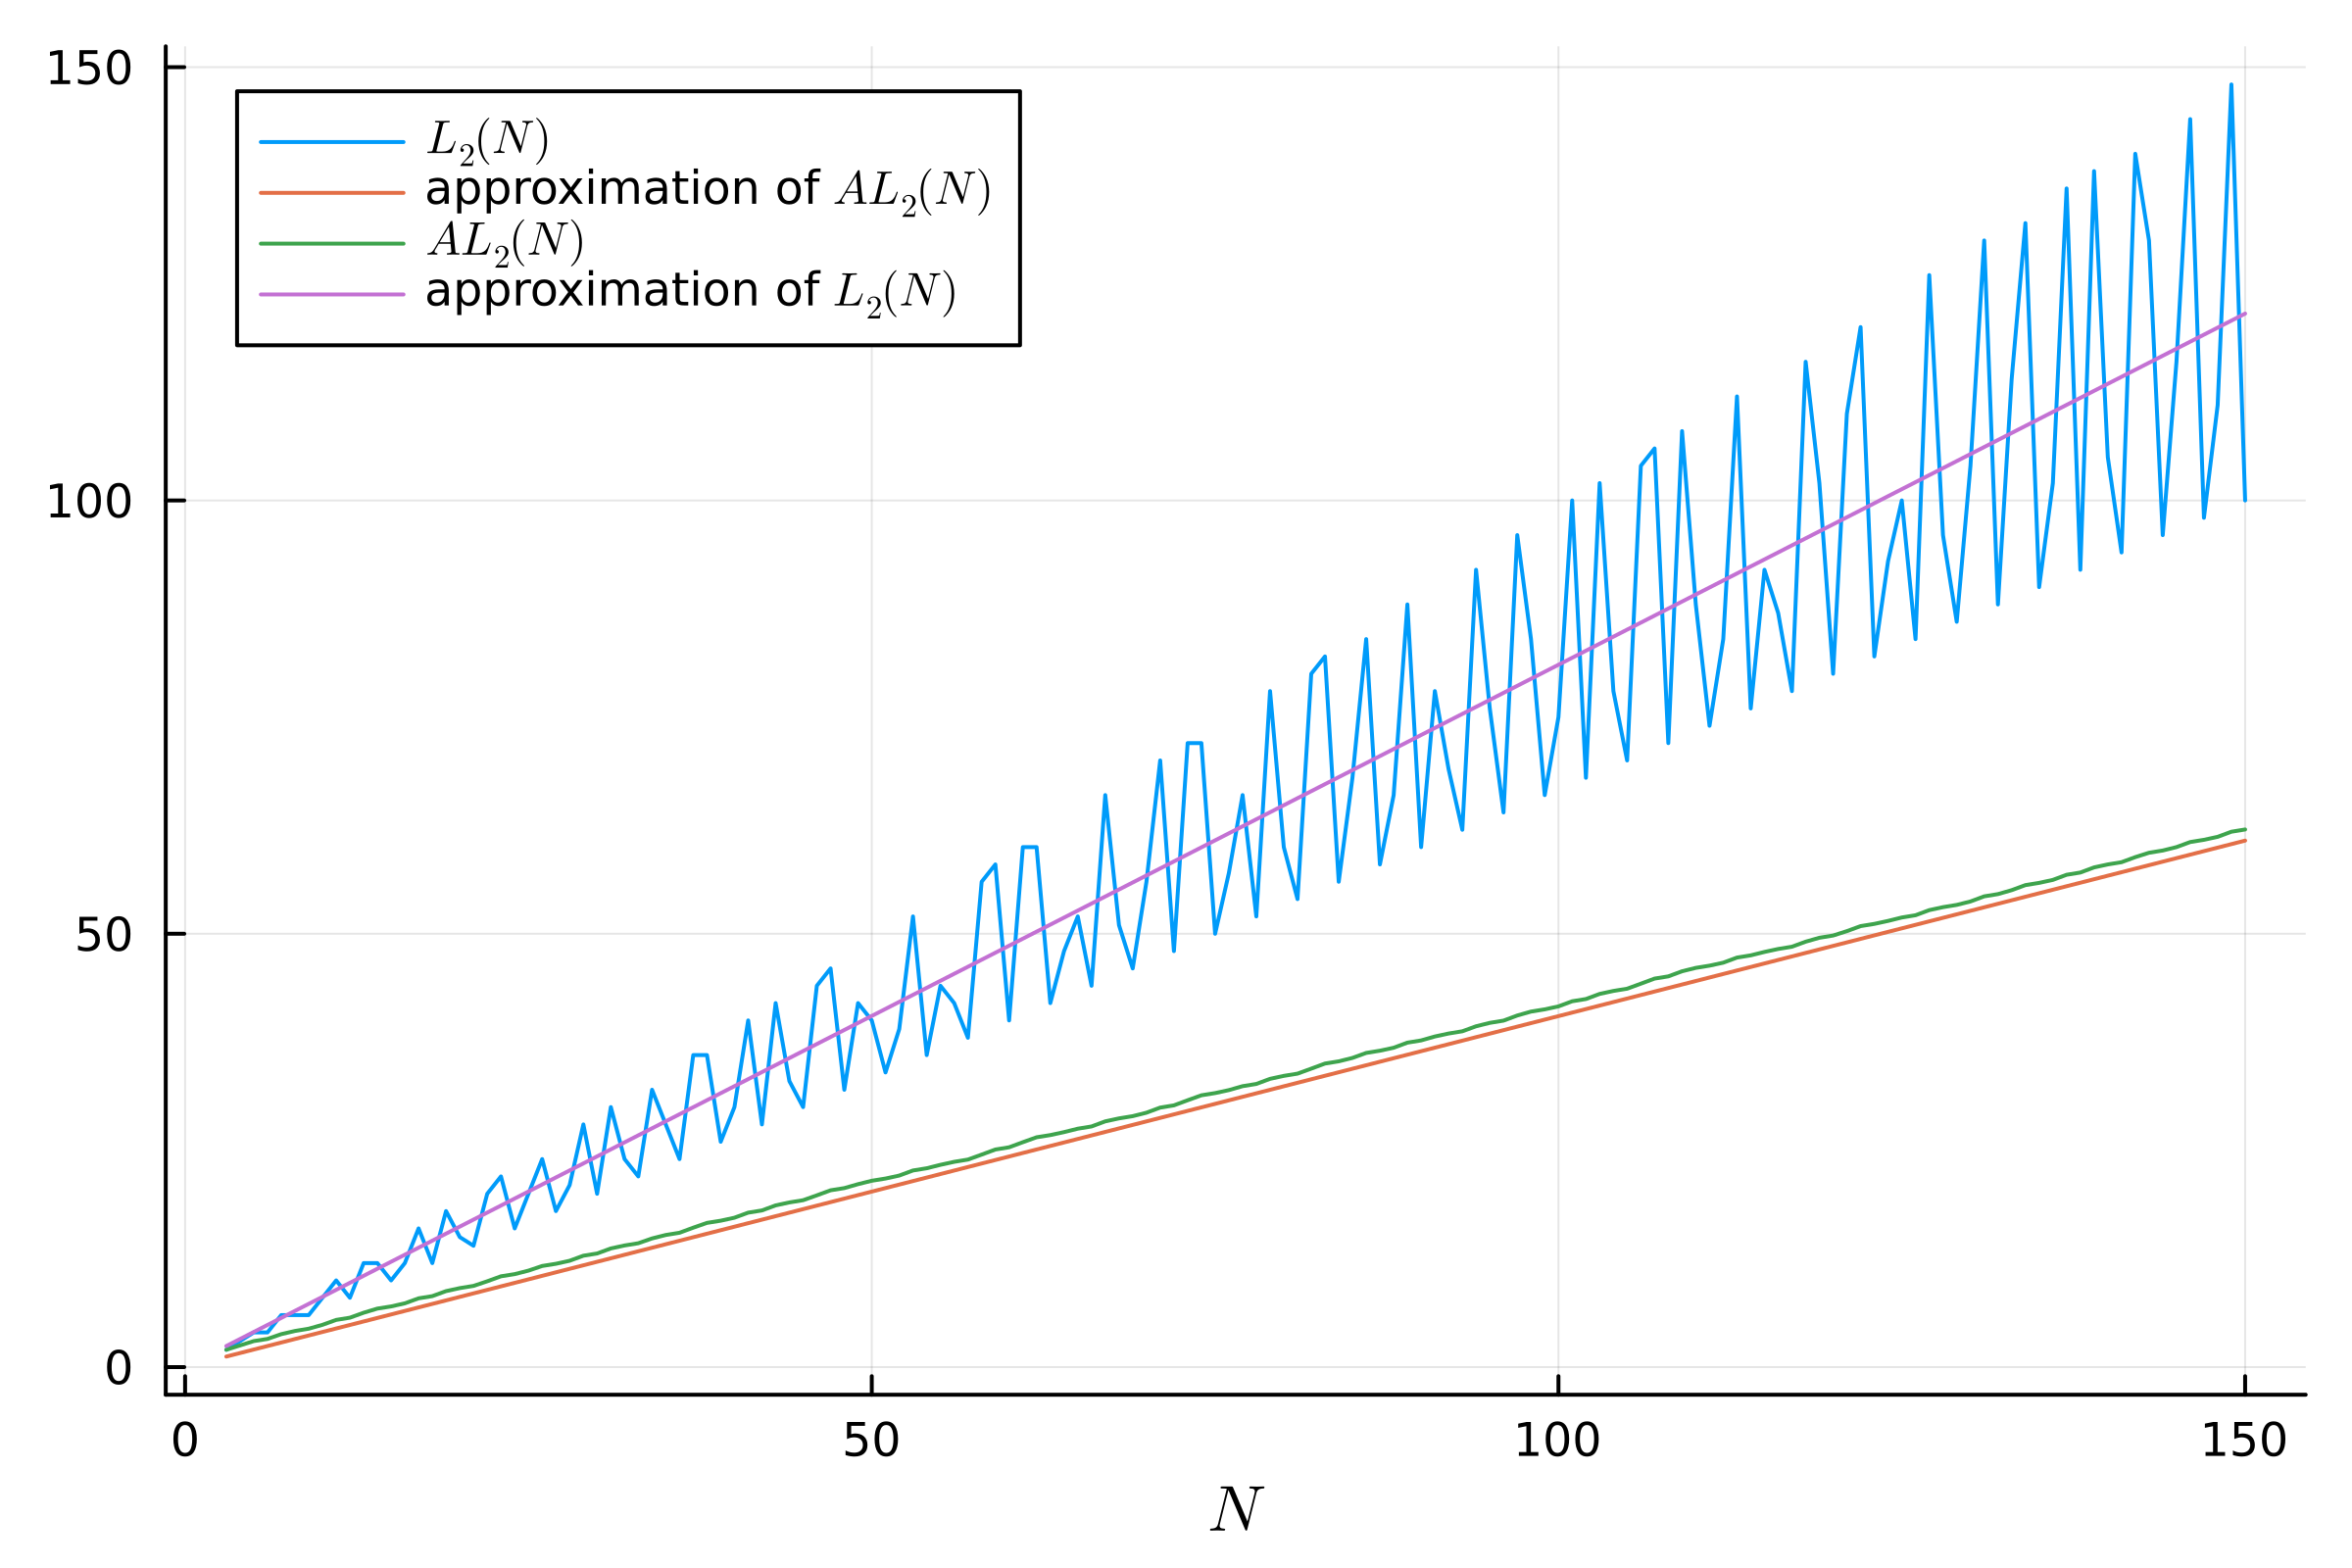
\includegraphics[width=\textwidth]{images/L_2_complete_analysis.png}
    \label{fig:figure1}
\end{figure}

\subsection{\(L_3(N)\) Case-wise Analysis}

Consider the simplest and most elementary situation where \(k = 3\). Now let one consider three situation for different possible congruences \(\mod 3\).

\begin{enumerate}
	\item If \(n \equiv 1 \pmod{3}\), then an example of a 3-partition could be \(1, k, 2k\) (with the sum exactly \(n\)) with a LCM of \(2k\), where \(n = 3k +1\), consequently we achieve an upper bound on the value for \(L_3(n)\) to be \(\frac{2(n - 1)}{3}\).
	\item If \(n \equiv 2 \pmod{3}\), analogously consider the example \(2, k, 2k\), again where \(n = 3k + 2\). As one can see, indeed the LCM is again \(2k\), thus again an upper bound is achieved of \(\frac{2(n - 2)}{3}\).
	\item Finally, if \(n \equiv 0 \pmod{3}\), then \(n = 3k\), let us again consider the possible congruences modulo \(3\) of \(k\). (As you can see the work for now is quite technical)
	\begin{itemize}
		\item If \(k \equiv 0 \pmod{3}\), then \(n = 9t\) and an example of \(t, 2t, 6t\) sets the upper bound of \(\frac{2n}{3}\)
		\item If \(k \equiv 1 \pmod{3}\), then \(3, k - 1, 2k - 2\) works, due to \(2k - 2 \equiv 0 \pmod{3}\)
		\item If \(k \equiv 2 \pmod{3}\), then \(6, k - 2, 2k - 4\) works, due to \(2k - 4 \equiv 0 \pmod{6}\) if \(k \equiv 2 \pmod{3}\)
	\end{itemize}
\end{enumerate}
Thus, indeed, one has established an upper bound on the value of \(L_3(N)\) to be \(\frac{2N}{3}\). It is important to note this bound is strict only for \(N\) large enough so that the above examples work (the exact number after which the bound starts working will be discussed a bit later). One can see the established lower and upper bound for the values of \(L_3(N)\),

\begin{figure}[h]
\centering
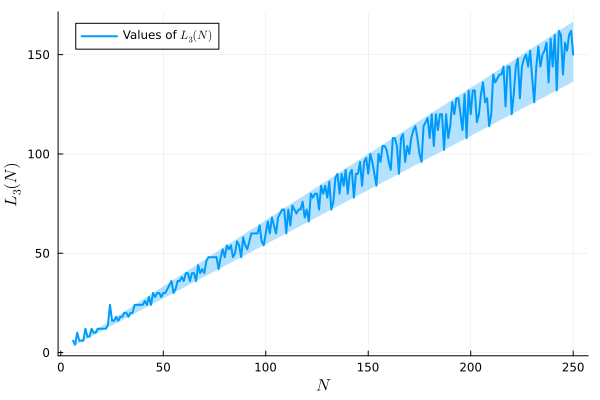
\includegraphics[scale=0.5]{images/L_3_plot}
\caption{}
\end{figure}

However, this somewhat brute-force approach does not work for larger values of \(N\), in fact already just to find an upper bound for \(L_4(N)\) posses a harder problem than before. Thus, calculating an upper bound for higher values of \(K\) requires a different perspective. In fact it seems the linear upper bound for \(L_4(N)\) while close, is not as tight as it was for \(L_3(N)\).

I want to note, that the value of \(L_3(N)\) is already to a large extend analysed, one already knows from the previous theorems, that \(\frac{6N}{11} \leq L_3(N) \leq \frac{2N}{3}\) (whilst, the upper bound is proven is a non-insightful fashion, it does not deminish the fact, that the bound is proven).

\subsection{Remarks on \(L_K(N)\)}

I cannot say much, about the completely generalized concept, except for the fact, that this problem is quite fundamental, if one thinks about it closer. Again, let us take a closer look at how can one interpret the value of \(L_2(N)\). Let us interpret all partitions of 2-partitions of \(N\), then one can easily come to see, that this is nothing more, than all the lattice points of a line \(y = -x + N\), thus if \(F_2(N) \geq L_2(N)\), this means, that for any line \(y = -x + N\), there exists a lattice point, which is less or equal to \(F_2(N)\), this interpretation can be easily generalized for larger dimensions.


\end{document}














































